\documentclass[conference]{IEEEtran}

\usepackage{algorithm}
\usepackage{algorithmic}
	
\usepackage{amsmath}
\usepackage{amsfonts}
	
\usepackage{graphics}
\usepackage{graphicx}

\usepackage{caption}
\usepackage{subcaption} 

\usepackage{hyperref}
\usepackage{verbatim}

\renewcommand{\L}{\mathcal{L}}

\usepackage{color}
\newcommand{\todo}[1]{{\small\color{red}[#1]}}

\renewcommand{\L}{\mathcal{L}}
\newcommand{\argmax}{\operatornamewithlimits{argmax}}

\usepackage{paralist}

%CHEAT CODES
%\renewcommand{\baselinestretch}{.99}
%\renewcommand{\textfloatsep}{0.5ex}

\begin{document}

\title{Zero-calibration BMIs for sequential tasks\\using error-related potentials}
%\title{Zero-calibration brain-machine interface: Learning labels and tasks with EEG-based feedback signals}

\author{\IEEEauthorblockN{Jonathan Grizou\IEEEauthorrefmark{1}, I\~naki Iturrate\IEEEauthorrefmark{2}, Luis Montesano\IEEEauthorrefmark{2}, Manuel Lopes\IEEEauthorrefmark{1}, Pierre-Yves Oudeyer\IEEEauthorrefmark{1}}
    \IEEEauthorblockA{\IEEEauthorrefmark{1} INRIA Bordeaux Sud-Ouest, France
    \\\{jonathan.grizou, manuel.lopes, pierre-yves.oudeyer\}@inria.fr}
    \IEEEauthorblockA{\IEEEauthorrefmark{2}Departamento de Inform\'atica e Ingenier\'ia de Sistemas (DIIS), Universidad de Zaragoza, Spain
    \\\{iturrate, montesano\}@unizar.es}
}

\maketitle

\begin{abstract}
Do we need to explicitly calibrate Brain Machine Interfaces (BMIs)? Can we start controlling a device without telling this device how to interpret brain signals? Can we learn how to communicate with a human user through practical interaction? It sounds like an ill posed problem, how can we control a device if such device does not know what our signals mean? This paper argues and present empirical results showing that, under specific but realistic conditions, this problem can be solved. We show that a signal decoder can be learnt automatically and online by the system under the assumption that both, human and machine, share the same a priori on the possible signals' meanings and the possible tasks the user may want the device to achieve. We present results from online experiments on a Brain Computer Interface (BCI) and a Human Robot Interaction (HRI) scenario.
\end{abstract}

\section{Motivation}
EEG-based brain-machine interfaces (BMIs) (see \cite{millan10} for a review) provide a communication channel between humans and machines using only brain activity. Since the first demonstration of brain-controlled devices, research on BMIs has emerged as one of the most growing research whose ultimate goal is endow with control capacities to people with severe motor disabilities. Yet, the practical promise of this technology remains unfilled with BMIs remaining confined to the laboratory or limited to clinical studies or home demonstrations that require close technical oversight \cite{sellers2010brain, lebedev2006brain}.

%Among the different brain recording techniques, electroencephalogram (EEG) has acquired increasing interest mainly due to its low cost and easiness of use. As a result, previous works have achieved successful control of complex systems such as real robotic devices and simulated agents, both with self-generated (e.g. motor imagery) and event-related (e.g. event-related potentials, ERP) signals (see \cite{millan10} for a review). 
%
Among the existent signals used to develop a BMI, recent works have shown that it is possible to decode information related to human error processing, namely the error-related potentials \cite{FerrezErrores} appearing for instance when the device action does not match the user's expectations. This potential has been used mainly to improve the BMI decoder \cite{Blumberg2007} and, more interestingly, as feedback information to solve sequential tasks \cite{chavarriaga2010learning, iturrate2010robot}. 
%
In fact, they can be interpreted as instructions given by a teacher to a learner under the implicit assumption that the two agents share a mutual understanding of feedback meaning (e.g. a decoder that translates raw signals into feedback such as speech into words).

In practice, BMI solves the meaning problem using an open-loop calibration procedure to train a decoder in a supervised manner. This calibration phase hinders the deployment of out-of-the-lab applications \cite{millan10}, due to the need of a specific calibration for each task and session. However, this phase is required mainly due to the non-stationary nature of the EEG \cite{vidaurre11}; the large intra- and inter-subject variability \cite{Polich1997}, and variations induced by the task \cite{IturrateErrP13}. 

It is worth noting this problem can be generalized to many kind of human-machine interaction (HMI) scenarios. In modern human-robot collaboration, there is a need for intuitive interfaces that allow non-technical users to teach robots. A major obstacle is that of requiring a pre-defined set of instruction signals. As a result, in the human to robot interaction (HRI) community, an important part of the work consists of building classifiers to translate human communicative signals (speech, gestures, facial expression) to symbolic meanings understandable by the robot. Such procedure requires a costly offline gathering of signals. A machine able to automatically understand such symbols could improve the usability and ease of use of such interactive system and even make use of involuntary signals, e.g. prosody, to better exploit the information provided by the user. 

While research on robot learning from human interaction has flourished in the last ten years \cite{Argall09lfdsurvey}, most work has focused on how to extract statistical \textit{task models} from human teachers following a fixed pre-defined teaching protocol. Thus, a usual assumption is that the learner and the teacher share a mutual understanding of the meaning of each others' signals. The question of how a robot can learn to interpret personalized and potentially noisy teaching signals, i.e.\ learn \textit{instruction models}, has been much less explored. In a preliminary work \cite{macl11simul}, we presented a computational approach addressing this problem by considering a finite space of symbolic teaching signals in simulation while bootstrapping the system with known symbols. Later \cite{grizou2013}, we released the need for bootstrapping and allow the teacher to use  signals that can be represented as fixed length feature vectors, which is better suited for HRI scenarios.

Interestingly, two similar approaches have been developed in the BMI community. In invasive BCIs, Orsborn et al. \cite{Orsborn2012} learned from scratch in closed loop a decoder for known targets using pre-defined policies to each target. However, the approach needed for a warm-up period of around 15 minutes. Similarly, Kindermans et al. proposed a method to reduce the warm-up period for non-invasive P300 signals by exploiting multiple stimulations and prior information \cite{Kindermans2012a,Kindermans2012b}.

In this paper we present a different approach to calibration procedures. We argue that, for some kind of problems, a calibration procedure is not explicitly needed. The system could learn, by interacting with the user, both what to do and how to map brain signals into meaningful instructions. The innovation of this work is not about new machine learning development but resides in a new way to use them. Our method combines and exploits two sources of information: task constraints and spacial organization of  instruction signals in the feature space. We report results from a BCI online experiments and a HRI scenario. The results show that the proposed method is able to learn good instruction models while solving the task efficiently without any prior calibration procedure.

%%%%
\section{Problem}

This section describes the problem of executing a task when the instruction signal's meaning is unknown or uncertain. For practical reasons, we will only refer to feedback driven BMI scenarios for the description of the problem and method. Nonetheless, the idea presented here holds for other HRI scenarios by replacing brain signals with other feedback instructions (e.g., speech). BMI control based on feedback signals (illustrated in figure~\ref{fig:grid}) differs from classical brain-machine interfaces in the sense that the user does not actively deliver commands to the device, but only delivers feedback about actions performed by the device. In this setting, the device needs to actively execute actions to solve the tasks and to be able to learn an intelligent behavior from the feedback. This idea can be seen as a shared-control strategy \cite{Iturrate13ErrPControl}, where both the user and the device help each other to solve a task.

\begin{figure}[!h]%
\centering
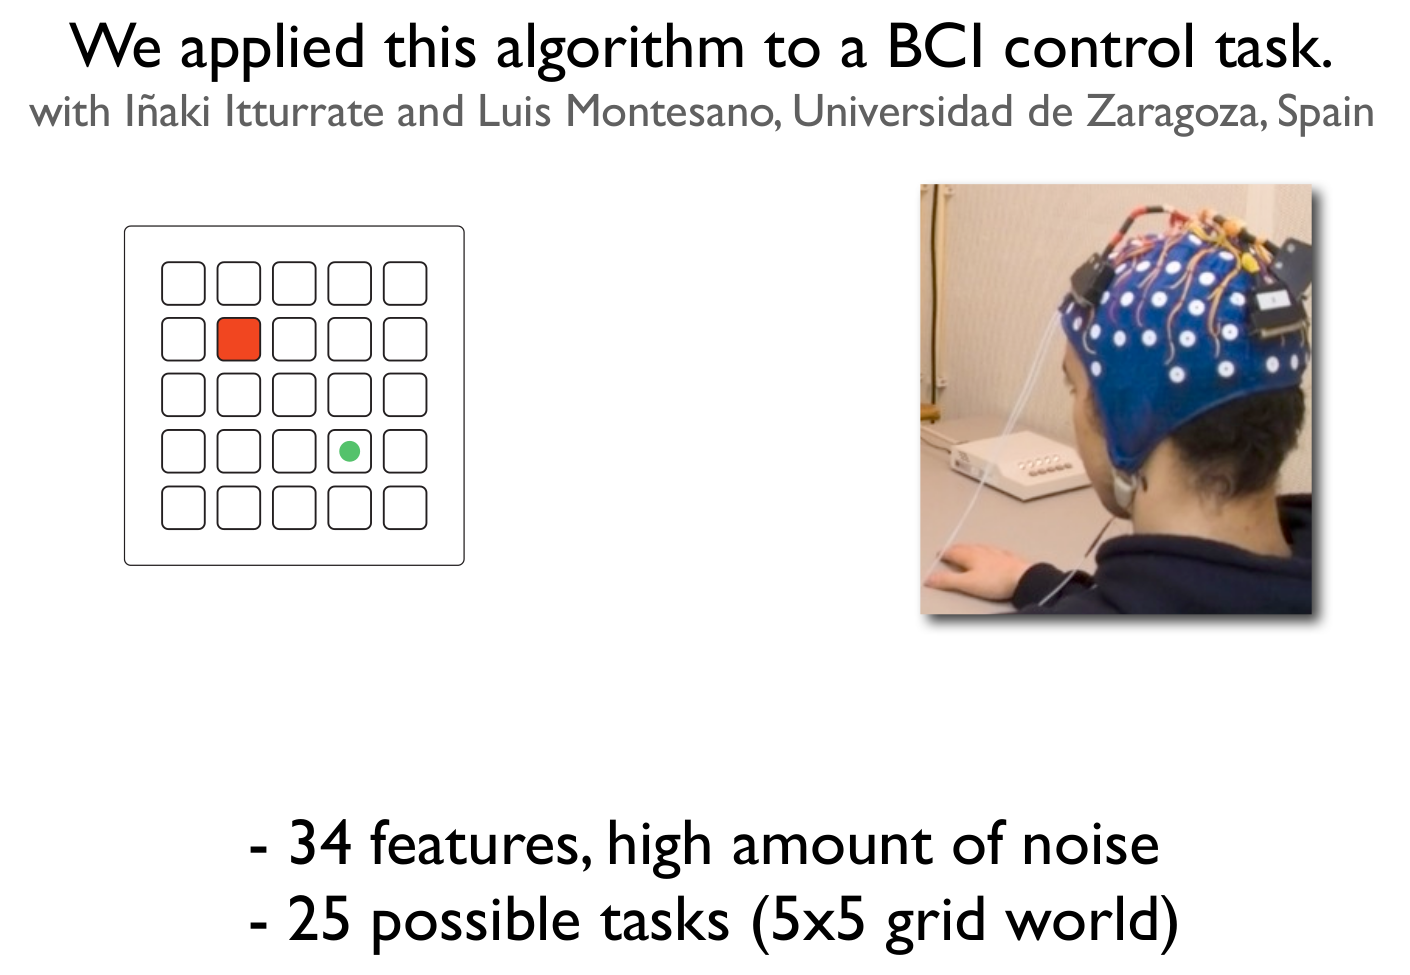
\includegraphics[width=1\columnwidth, trim=3cm 12cm 3cm 6cm, clip=true]{images/BCI.png}
\caption{In this BMI scenario, the user is watching the agent moving on the screen and assess the agent actions with respect to its own objective illustrated by the red state.}
\label{fig:grid}
\end{figure}


Essentially, this BMI control follows an iterative sequential process where, in a particular state $s$, the device performs an action $a$ and the user assesses the action using brain signal $e\in\mathbf{R}^n$. These assessments generate error-related potentials, i.e. signals elicited in the brain when the outcome observed by the user differs from the expected one \cite{FerrezErrores}. Thus, collected data are in the form $\{(e_i,s_i,a_i),~i~=~1,\ldots,N\}$, i.e. a sequence of states, actions and teaching signals triplets, with $N$ the number of steps. 
%
In a common scenario, the system has been fed with a classifier, parameterized by $\theta$, that translates brain signals $e$ into symbolic instructions $z$ that belong to one of two classes (correct or incorrect assessment), $z\in\{c,w\}$. The model parameters $\theta$ are in practice learnt using a calibration procedure. The device then learns from this symbolic feedback. 

%After a calibration phase and once a usable decoder, represented by a set of parameters $\theta$, is available, these assessments $e$ are translated into symbolic feedback $z\in\{c,w\}$ that belong to one of two classes (correct or incorrect), and the device learns from this feedback.

This control can be exemplified for a reaching task (Fig.~\ref{fig:grid}), where the user wants to reach a target position unknown by the system. The device performs several discrete actions (e.g. moving left or right), and learns from the feedback given by the user. After several steps, the device knows which is the desired target and how to reach it.
%
However, the control can become intractable as the task complexity increases. Furthermore, only binary feedback is available and there is a large percentage of misdetected assessments. Given a set of possible tasks $\Xi$ = \{$\xi_1, \ldots, \xi_T\}$, with $T$ the number of task hypothesis, it is possible to speed up the inference by precomputing the agent's optimal behavior $\pi_{\xi} = p(a|s,\xi)$ for each task and using the feedback signal as a likelihood for the task.  For instance, in the previous example, the possible tasks are given by the number of targets. This way, an error (negative feedback) after a particular action will decrease the posterior probability of those targets whose optimal policy agrees with the action.

In this work, we address the problem of removing the need for calibration. Therefore we do not have access to the negative or positive nature $z\in\{c,w\}$ of the brain signals $e$ beforehand. We propose an algorithm that simultaneously calibrates the feedback decoder and executes in closed loop a sequential task only known by the user $\hat{\xi} \in \Xi$ . Our method combines and exploits two sources of information: task constraints, namely optimal policies $\pi_{\xi}$, and spatial organization of brain signals in the feature space. The underlying assumptions are: 

\begin{inparaenum}
\item a finite number of possible task hypothesis, i.e. $\xi_l$ for $l \in {1,\ldots,\xi_T}$, can be defined 
\item the inputs signals have some hidden labels $z$ corresponding to their meaning
\item the set of possible meanings is finite, e.g. $z \in \{c, w\}$
\item given the ground truth labels $\hat{z}$ of the signals, a classifier of sufficient accuracy could be trained to control the device.
\end{inparaenum}

These assumptions may look constraining but are actually common ones in most current BMI scenarios. For example, consider the case of a robotic arm assistant helping to grasp objects on a table. Such robotic assistant could be controlled by a user assessing the robot actions. For instance, the robot could start reaching for an object having the user validating or not the decision of the robot. In such scenario, the usual method would be to start a calibration procedure to map ERP brain signals into symbolic feedback instructions for the robot (correct and incorrect). Once enough data are collected, a classifier would be trained and we could start assessing the robot's actions using brain ERP. This simple scenario, which follows a calibration procedure, already includes all the assumption we defined earlier. We have 
\begin{inparaenum}
\item a finite set of hypothesis represented by the finite number of object on the table
\item a user that is told to assess the robot's actions
\item a finite set of possible meanings (correct and incorrect)
\item signals that can be classified as the calibration procedure was able to generate a usable classifier.
\end{inparaenum}
%
\section{Method}
%
This section describes our proposed solution to the previously defined problem of executing a task when the instruction meaning is unknown or uncertain and under the given assumption. The main idea is depicted in Fig. \ref{fig:GM} for a toy 1D example. The user wants the device to reach the right-most state. However, neither the target $\hat{\xi}$ nor the true feedback labels $\hat{z}$ are known. The feedback signals $e$ are generated as a response to the execution of an action $a$ in state $s$ according to the true unknown task $\hat{\xi}$ the user wants to solve.  The key point is that  these signals are generated from an underlying model that for binary signals has two different classes. Given sufficient feedback signals, it is possible to build the underlying distributions for each possible target. Only the right task will provide the right meanings (or labels) to each of the feedback signals (Fig. \ref{fig:GM}~Left), while the other tasks will gradually mix both classes as the task gradually differs more from the original task (Fig. \ref{fig:GM}~Middle-Right), up to the point of almost mirroring the labels when the target is mirrored. In the remainder of this section we show how this property can be exploited to estimate the task and the model generating the feedback signals.

\begin{figure}[!h]%
\centering
\includegraphics[width=1\columnwidth]{images/real_vs_fake}
\caption{Task-dependent labels for a 1-D grid world.  For the represented example, the arrows indicate for each state what action should elicit a positive feedback to reach the target marked with T (i.e., the optimal policies). 2D Gaussian distributions of binary feedback signals for three possible targets are shown below. While for the correct target the distributions shows a large separability (Left), the overlaps increases as the believed target moves away from the real one (Middle, Right). }
\label{fig:GM}
\end{figure}


Following the literature \cite{blankertz2010single}, we will model the EEG signals using independent multivariate normal distributions for each class, $\mathcal{N}(\mu_c, \Sigma_c), \mathcal{N}(\mu_w, \Sigma_w)$. Here, the model parameters $\theta$ account for $\{\mu_c, \Sigma_c,\mu_w, \Sigma_w\}$. 

Regarding the tasks, the system has access to a set of task hypotheses $\Xi$ which includes the task  $\hat{\xi}$ the user wants to solve\footnote{If this is not the case, the system will find the most suitable task.}. We do not make any particular assumption on how the task is represented given that for each particular task $\xi$ we are able to compute a policy $\pi_{\xi}$ which represents the probability of choosing a given action $a$ in state $s$, $\pi_{\xi}(s,a) = p(a|s,\xi)$. These policies, conditioned on the task, provide meanings to the signals of an action-state pair (e.g. in a reaching task, progressing towards the goal will generate correct answers while moving apart from it will generate wrong ones). We define $Z$ the function that, given a state $s$, an action $a$, and a task $\xi$ return the probability of the user intended meaning $z$, i.e. $Z(s,a,\xi) = p(z|s,a,\xi)$. With $\sum_{f=c,w} p(z=f|s,a,\xi) = 1$. Instead of a binary meaning estimate, we add a noise term to cope with those situations were the user assessment may be wrong.  For example, the probability that the user, having task $\xi$ in mind, provides a signal of meaning correct $c$ if the device execute action $a$ in state $s$ is:
%
\begin{equation*}
    	p(z=c|s,a,\xi) =
     	\begin{cases}
		1-\alpha          & if~a = \argmax_a \pi_{\xi}(s,a)\\
		\alpha             & \text{otherwise}\\
	\end{cases}
\end{equation*}
with $\alpha$ modeling error rate of the user. In our case, only two signal meanings are possible, i.e. correct ($c$) and incorrect ($w$), therefore: $p(z=w|s,a,\xi) = 1- p(z=c|s,a,\xi)$

Following the discussion of Fig. \ref{fig:GM}, a sensible option to estimate the task $\hat{\xi}$ is to measure the coherence of the signal model $\theta_\xi$ computed using the virtual meanings, given by $Z$, provided by the target policy. In other words, the best $(\xi,\theta_{\xi})$ pair would provide the lowest predictive error (perr) on the observed signals $p(e|s,a,\xi,\theta)$. One possible way of solving this problem is to maximize the expected predictive classification rate:
%
\begin{eqnarray}
\hat{\xi},\hat{\theta}&=& argmax_{\xi,\theta}~E_e\left( \delta(Z(s,a,\xi), Y(e,\theta_\xi)) \right)
\end{eqnarray}
where $\delta()$ being an indicator function. And $Y(e, \theta_\xi)$ is the predicted label $z$ for signal $e$ under the model parameterized by $\theta_\xi$, i.e. $Y(e, \theta_\xi) = p(z|e, \theta_\xi)$. With $\sum_{f=c,w} p(z=f|e, \theta_\xi)=1$.  In practice, it is just the probability of the meaning under the Gaussian model provided by $\theta_{\xi}$. For example, the probability that signal $e$ is of meaning correct ($c$) under $\theta$ can be expressed as:
%
\begin{eqnarray}
	p(z=c|e,\theta) &=& \frac{p(e|z=c, \theta)p(z = c)}{\sum_{k=c,w}{p(e|z=k,\theta)p(z=k)}}\nonumber\\
			&=& \frac{\mathcal{N}(e|\mu_c, \Sigma_c)p(z = c)}{\sum_{k=c,w}{\mathcal{N}(e|\mu_k, \Sigma_k)p(z=k)}}
	\label{eq:dev}
\end{eqnarray}
In our case, only two signal's meaning are possible, i.e. correct ($c$) and incorrect ($w$), therefore: $p(z=w|e,\theta) = 1-p(z=c|e,\theta)$.

The expected predictive error can be explicitly written dependent on the task and decoder model:
%
\begin{eqnarray}
E_e\left( \delta(Z(s,a,\xi), Y(e,\theta)) \right)  &=&  \nonumber \\ \sum_{f=c,w} p(z=f|s,a,\xi) p(z=f|e,\theta)
%E_{e \sim \theta,\xi}
\end{eqnarray}

Note that the optimization process has been factored using the fact that given a task $\xi$, the estimation of $\theta$ under the Gaussian model is trivial. It basically requires to compute the maximum-likelihood estimate $\theta^{ML}_{\xi}$ for each task $\xi$. 

Concretely, given a set of task hypothesis $\Xi$ of size $T$, we can assign, for each hypothesis, probabilistic labels to the signals received from the user ($Z$). This provides one dataset of signals with $T$ sets of labels. For each task hypothesis and given its associated hypothetic label set, we can now compute the maximum-likelihood model $\theta^{ML}$. By comparing the fitted model prediction ($Y$) with the initially assigned labels ($Z$), we can compute a score, here  the expected predictive error, that account for the coherence of the spacial organization of brain signals in the feature space with the associated hypothetic labels. The idea is that only the right task will provide the right meanings (or labels) to each brain signals, while the other tasks will gradually mix both classes (Fig. \ref{fig:GM}). The correct task should therefore have a lower expected predictive error.

\section{Results}

In this section we present online results from a BCI scenario as well as a pick and place HRI scenario to illustrate the wider potential application of our approach. For the remaining of this section, we will consider the error rate of the user $\alpha$ equals to $0.1$.

\subsection{BCI Control Task}

\subsubsection{Control task}
As illustrated in figure~\ref{fig:grid}, we consider a 5x5 grid world, where an agent can perform five different discrete actions: move up, down, left, right, or a target-reached action. The user goal is to teach the agent to reach one, yet unknown to it, of the $25$ discrete positions which represent the set of possible tasks. We thus consider that the agent has access to 25 different task hypothesis (one with goal location at each of the cells). We use \textit{Markov Decision Processes} (MDP) to represent the problem \cite{sutton1998reinforcement}. From a given task $\xi$, represented as a reward function, we can compute the corresponding policy $\pi_{\xi}$ using, for instance, Value Iteration \cite{sutton1998reinforcement}. 
%There are no ambiguities due to the presence of a target-reached action.
%
\subsubsection{EEG-based feedback signals}
%
EEG signals were recorded with a gTec system (2 gUSBamp amplifiers) with 32 electrodes distributed according to the 10/10 international system, with the ground on FPz and the reference on the left earlobe. The EEG signals were digitized with a sampling frequency of $256$ Hz, common-average-reference (CAR) filtered and band-pass filtered at $[0.5, 10]$ Hz. 

During operation, the role of the users was to assess the agent actions as good or bad, obtaining this way potentials associated to correct or erroneous actions. Previous studies have demonstrated that these signals can be detected online \cite{FerrezErrores} and even be used as binary feedback signals \cite{chavarriaga2010learning}. Following these studies, features were extracted from two fronto-central channels (FCz and Cz) within a time window of $[200,700]$ ms (being 0 ms the action onset of the agent) and downsampled to $32$ Hz. This leaded to a vector of $34$ features. This feature vector served as the input for our algorithm
%
\subsubsection{Zero-calibration BCI Control with Human Subjects}
%
This experiment will evaluate the main claim of our algorithm, that we can identify the task desired by the user even without an explicit calibration phase and without any knowledge of the brain signals. The experiments were conducted with four subjects (aged between $25$ and $28$). Each subject performed $5$ runs of learning from scratch how to reach a target (chosen randomly).

Figure \ref{fig:online_results} summarizes the results. The probability of the correct task (averaged across subjects and tasks) is shown in Fig \ref{fig:online_results}a. Figure \ref{fig:online_results}b shows the run by run results. We can conclude that the algorithm is very robust as all the subjects were able to identify the correct task. There are strong variations among subjects, but we note that in previous works the calibration phase used between  300 and 600 examples \cite{chavarriaga2010learning, iturrate2010Katana}. Thus, even for the worst subject, it is still possible to start controlling the system without calibration and in less iteration than required by such calibration procedure. 

\begin{figure}[!htbp]
	\centering
		\begin{subfigure}[t]{1\columnwidth}
			\centering
   			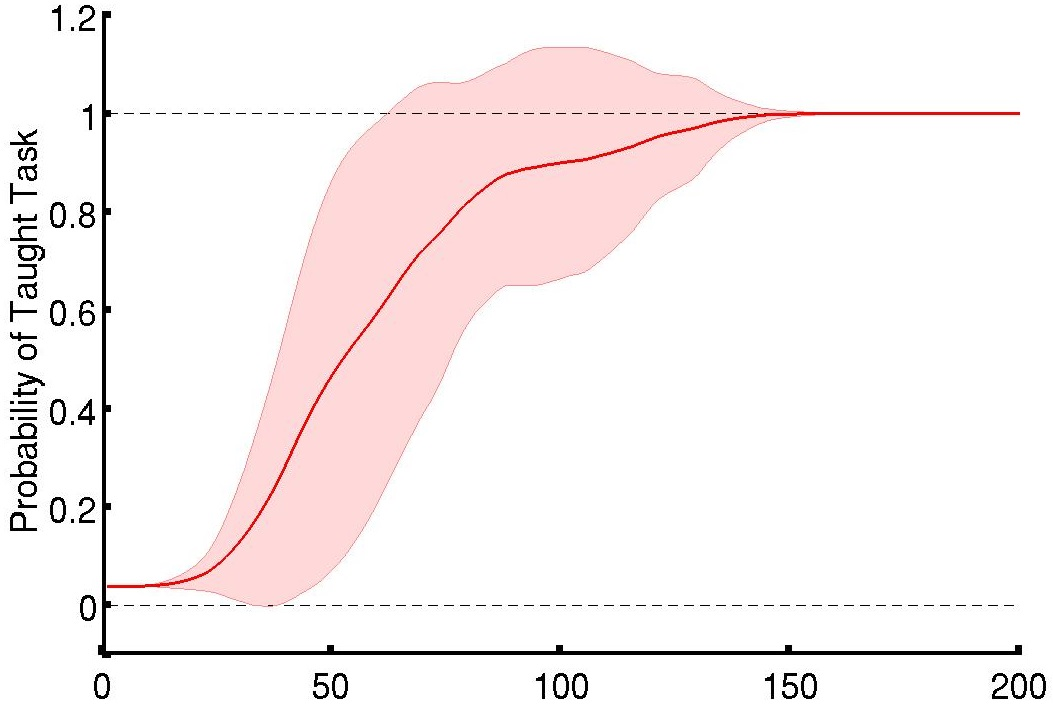
\includegraphics[width=\columnwidth]{images/Avg_evo_likelihood.jpg}
   			\caption{} 
			\label{fig:avg_evo_real}
		\end{subfigure}
		\begin{subfigure}[t]{1\columnwidth}
			\centering
   			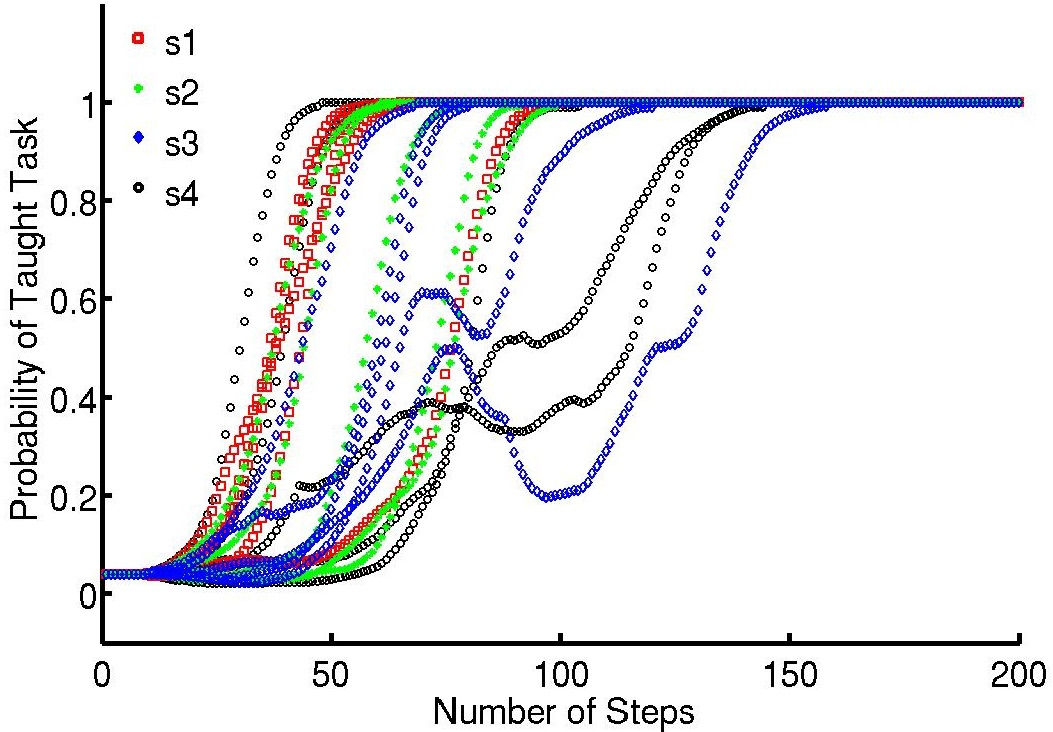
\includegraphics[width=\columnwidth]{images/Evo_likelihood.jpg}
   			\caption{} 
			\label{fig:subject_evo_real}
		\end{subfigure}
	\caption{\label{fig:online_results} Results from the online BCI experiment for identifying the task: a) Evolution of the probability of the taught task averaged for all subjects; b) Evolution of the probability of the taught task for each subject and run} 
\end{figure}

\subsection{HRI Pick and Place scenario}

In this section, we illustrate the broad range of possible application for our approach with a small size pick-and-place task with a real robot. This robot is going to be programmed using a natural speech interface whose words have an unknown meaning and are not transformed into symbols via a voice recognizer. The interaction between the robot and the human is a turn taking social behavior, where the robot performs an action and waits for a feedback instruction signal to continue. This allows to synchronize a speech wave with its corresponding pair of state and action. 

\subsubsection{Experimental System}

We consider a six d.o.f. robotic arm and gripper that is able to grasp, transport and release cubes in four positions. We used a total of three cubes that can form towers of two cubes.  The robot has 4 actions available: \textit{rotate left}, \textit{rotate right}, \textit{grasp cube} and \textit{release cube}. The state space is discrete and defined as the location of each object, including being on top of another or in the robot's hand. So for a set of 3 objects we have 624 different states. Figure~\ref{setup} shows the robot grasping the orange cube. 

As for the BCI control task, MDP is used to represent the problem. For this particular representation we assume that the reward function is sparse and so we can generate possible tasks by sampling sparse reward functions. In other words the task is to reach one, yet unknown, of the 624 states of the MDP.

\begin{figure}[!t]
	\centering
		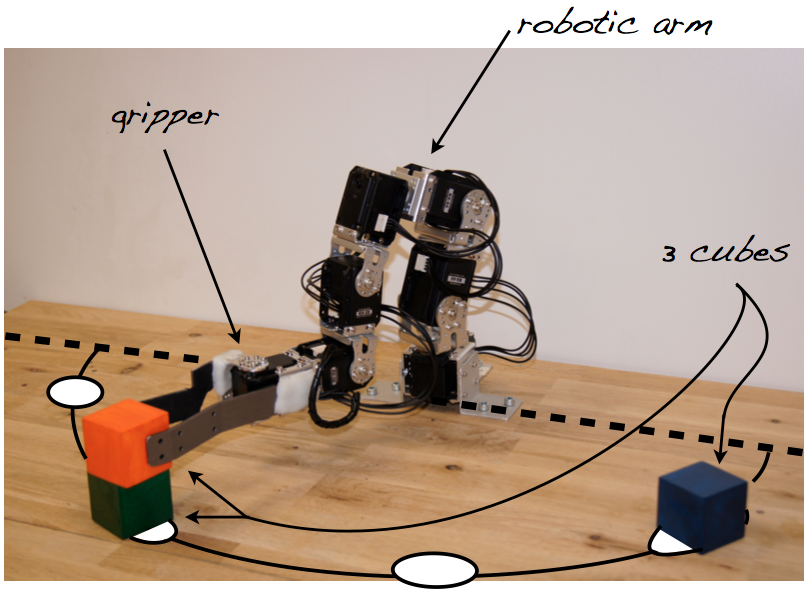
\includegraphics[width=0.7\columnwidth]{images/setup4.png}
	\caption{Robotic System. A six d.o.f robotic arm and gripper learning to performing a pick-and-place task with three cubes.}
	\label{setup}
\end{figure}

\subsubsection{Speech processing}

We consider speech as the modality for interacting with the robot. After each action we record the teaching word pronounced by the user. This data is mapped into a $20$ dimensional feature space using the methodology described next.  

A classical method for representing sounds is the \textit{Mel-Frequency Cepstral Coefficients} (MFCC) \cite{zheng2001comparison}. It represents a sound as a time sequence MFCC vectors of dimension $12$. Comparing sounds is done via \textit{Dynamic Time Warping} (DTW) between two sequences of feature vectors \cite{sakoe1978dynamic}. This distance is a measure of similarity that takes into account possible insertions and deletions in the feature sequence and is adapted for sounds comparison of different length. Each recorded vocal signal is represented as its DTW distance to a base of 20 pre-defined spoken words which are not part of words used by the teacher.

By empirical test on recorded speech samples, we estimate that a number of 20 bases words were sufficient and yet a relatively high number of dimensions to deal with a variety of people and speech. This base of 20 words has been randomly selected and is composed of the words:\emph{ \footnotesize{Error, Acquisition, Difficulties, Semantic, Track, Computer, Explored, Distribution, Century, Reinforcement, Almost, Language, Alone, Kinds, Humans, Axons, Primitives, Vision, Nature, Building}}.

It should be made explicit that this is not state of the art speech processing technics but is not the concern of our research. This representation allow to represent spoken words in a relatively low dimensional space with good accuracy.

\subsubsection{Zero-calibration HRI online pick and place experiment}

This brief experiment demonstrates the transferability of our approach to other domains. In addition, it briefly illustrates the ability of our algorithm to reuse acquired knowledge. Once the robot has understood the first task, we can freeze the classifier corresponding to the identified task and start learning a new task faster as this time the signal to meaning mapping is known.

\begin{figure}[!h]
	\centering
		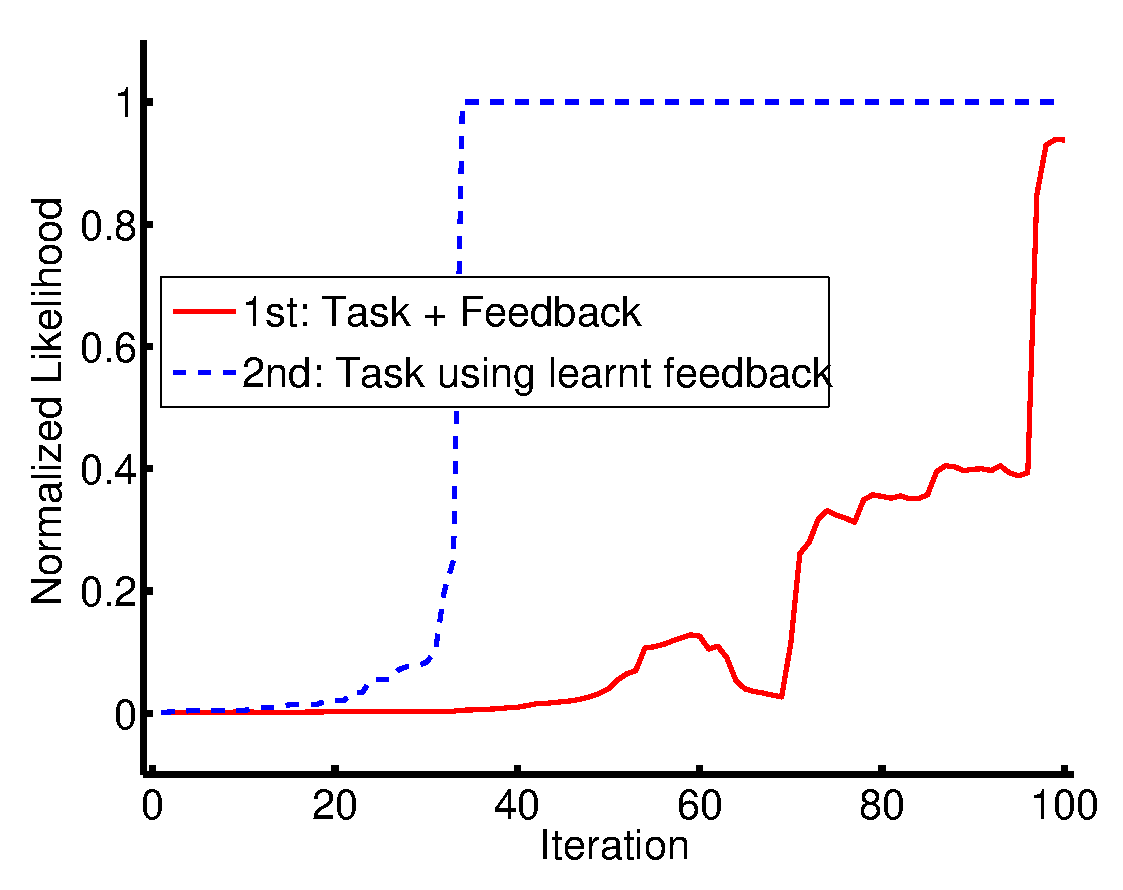
\includegraphics[width=0.9\columnwidth]{images/real}
	\caption{Evolution of the probability of the taught task. 1) The robot learns a task from unlabeled speech feedback. 2) By freezing the classifier corresponding to the best task estimate, the user teaches the robot a new task faster.}
	\label{Real}
\end{figure}


Fig.~\ref{Real} shows results from one online interactive session with a user using speech to teach the robot what configuration of cube it wanted to the robot to build. In the first run it takes about 100 iterations for the robot to learn the task. Whereas in the second run, when reusing knowledge from the first one, the robot is able to learn a new task faster, in about 30 iterations, meaning that it has well found the two clusters in our feature space as well as the mapping to their corresponding meanings.


\section{Discussion}

For communication to be successful, the human and the machine need to share some common background which is usually the meaning of the signals received by the device. In practice, such signal to meaning mapping is represented by a specific classifier learnt using a calibration procedure. In this work we have seen that this signal-to-meaning classifier can be learnt automatically and online by the system under the assumption that both, human and machine, share the same a priori on the possible meanings of the signals and the possible task the user may want the device to achieve. We presented a learning algorithm able to associate meaning with unknown signals by reasoning about their relation to previous signals and their relation to the environment itself. The intuition for our method is that the classification of the brain/speech signals is easier when they are interpreted according to the task desired by the user. The method thus relies on finding which pair of classifier-task has the smaller expected prediction error in the signals. We considered the case of brain signals but of particular interest is the possibility to use the same system with other modalities, such as speech. This allows different users to use the system according to their own preferences, skills and limitations. Finally, we tested our algorithm with real users and showed that, once the system has identified a first task, it can reuse the acquired knowledge about the user instruction signals for learning of a new task faster.
%knowledge acquired from a first experiment can be reused later as a source of known information
%Importantly, once the system has identified a first task, it can reuse the acquired knowledge about the user instruction signals for learning of a new task faster. 

An important challenge for such interactive systems is to deal with non-expert humans. Several studies discuss the different behaviors naive teachers use when instructing robots \cite{Thomaz2008,Cakmak2010}. An important aspect is that the feedback is frequently ambiguous and deviates from the mathematical interpretation of a reward or a sample from a policy. For instance, in the work of \cite{Thomaz2008} the teachers frequently gave a positive reward for exploratory actions even if the signal was used by the learner as a standard reward. Also, even if we can define an optimal teaching sequence, humans do not necessarily behave according to those strategies \cite{Cakmak2010}. Such aspects were not further considered in this work than by modeling the error-rate of the user.

We believe working without calibration procedure is a novel challenge that can make human to machine interaction more practical to use. Future work will consider how the device can act in order to disambiguate faster the different hypotheses. An important direction is to push this method towards more advanced robotic scenarios by considering, for example, continuous state-action spaces, asynchronous interactions and more complex types of instructions.

\newpage

\section*{Acknowledgements}
The authors from INRIA are with the Flowers Team, a INRIA / ENSTA-Paristech joint-lab. The research reported was (partially) supported by INRIA, Conseil R\'egional d'Aquitaine and the ERC grant EXPLORERS 24007.

\bibliographystyle{IEEEtran}
\bibliography{ref}


\end{document}








\section{Discussion}

Learning how to communicate with a human user through practical interaction. The learning algorithm is able to associate meaning with unknown inputs by reasoning about their relation to previous input and their relation to the environment itself.

We believe working without calibration procedure is a novel challenge that can make Human to Machine Interaction more practical to use.

We have seen that under some application constraints it is possible to calibrate a system online and while controlling the device.

The intuition for our method is that the classification of the brain/speech signals is easier when they are interpreted according to the task desired by the user. The method thus relies on finding which pair of classifier-task has the smaller expected prediction error in the signals. 

The innovation of this work is not about new machine learning development but reside in a new way to use them. 

A combination of constraints applied by the task and the signal meaning with machine learning algo makes it possible to remove the calibration task.
Aside from this conceptual contribution we also identified a way for the device to actively select it action in order to identify the signals and task faster.

If one unique idea should be remembered. It is not the technics, the algorithm detail neither the practical experiment conducted here that should be remembered but the new problem defined here and the constraints and assumption that allow to solve it resulting in more flexible, intuitive, way of starting interacting with a device, a robot or any systems thought practical interaction under the assumption that the signals used are differentiable, the interaction context can be reduce to a finite set of hypothesis, the meaning of the signals are known in advance. Such assumption are made explicit in this work but are in fact most of the assumption that actually holds in most BCI or BRI setup. A classifier is trained using a calibration procedure, which prove the data can be classified. The user is told to think about yes or no or left hand right leg movement, which will be mapped to a specific finite set of possible meaning. Finally in most particular scenario, e.g. grasping one object on a table, the context in which the device is used allow to identify a finite set of possible task, action the user may want the user to accomplish.

For communication to be successful, the human and the machine need to share some common background which is usually the meaning of the signals received by the device. In practice, such signal to meaning mapping is represented by a specific classifier learnt using a calibration procedure. In this work we will see that this signal to meaning classifier can be learnt automatically and online by the system under the assumption that both, human and machine, share the same a priori on the possible meanings of the signals and the possible task the user may want the device to achieve.
example from a HRI and BCI experiment. 
the structure in the data in combination with tasks constraints

We did not discussed the action selection method used by the robot/device. An interesting problem is how the robot can act actively in this kind of problem.



The main idea behind this work is that, under specific constraints and assumption which often applies in BMI scenario, one can allow a user to interact with a machine without the need of an expert calibrating the system. Resulting in a more flexible and intuitive way of starting interacting with a device to solve sequential tasks.








Our method exploits task constraints, namely optimal policies, to hallucinate the meaning of the teaching signals and select the task with the lowest expected error. 

Related work on this domain is very limited. Griffiths et al. \cite{griffiths2012bottom} conducted an experiment with human learning the meaning of unknown symbolic teaching signals. 

In this abstract, we address the problem of removing the need for calibration. We propose an algorithm that simultaneously calibrates the feedback decoder and executes in closed loop a sequential task only known by the user. Our method exploits task constraints, namely optimal policies, to hallucinate the meaning of the teaching signals and select the task with the lowest expected error. We report results from a HRI scenario and a BCI online experiments. The results show that the proposed method is able to learn good feedback models while solving the task efficiently without any calibration.


%Among the different issues that limits the home use of BMIs  \cite{sellers2010brain} is the need for an expert calibrating and re-calibrating the system as the task or the brain signals changes. The need for specific calibration is required mainly due to the non-stationary nature of the brain signals \cite{vidaurre11}; the large intra- and inter-subject variability \cite{Polich1997}, and variations induced by the task \cite{IturrateErrP13}.





This calibration phase hinders the deployment of out of the lab applications \cite{millan10}, due to the need of a specific calibration for each task designed by an expert. 

 areas in part due to its potential to improve the lives of disabled people. The ultimate goal of BMIs technology is to provide communication and control capacities to people with severe motor disabilities. 


Note that the same task could be performed with the robot actions being evaluated as correct or incorrect by the user.

the decoder that transform signals into meaningful instructions 

In this work we address the problem of removing the need for calibration.

Interestingly, the need to create decoders that transform signals into meaningful instruction to program a machine is of wider application. 




More gene

neural sciences and robotics are growing

Interfacing brain signals recording to robots or computers is a laborious process that requires a long and fastidious calibration procedure. 
\cite{sellers2010brain}
\cite{lebedev2006brain}
This is a major problem
As a result, a limited amount of BCI or BRI systems are used by people outside of the lab. requires an expert to collect and train the classifier. The recording devie need to be placed at the exact same location or the all calibration should be started again. 
In this work
The learning algortihm involved are state of the art classifier and RL technics.


%\begin{figure}[!t]
    %\begin{center}
           %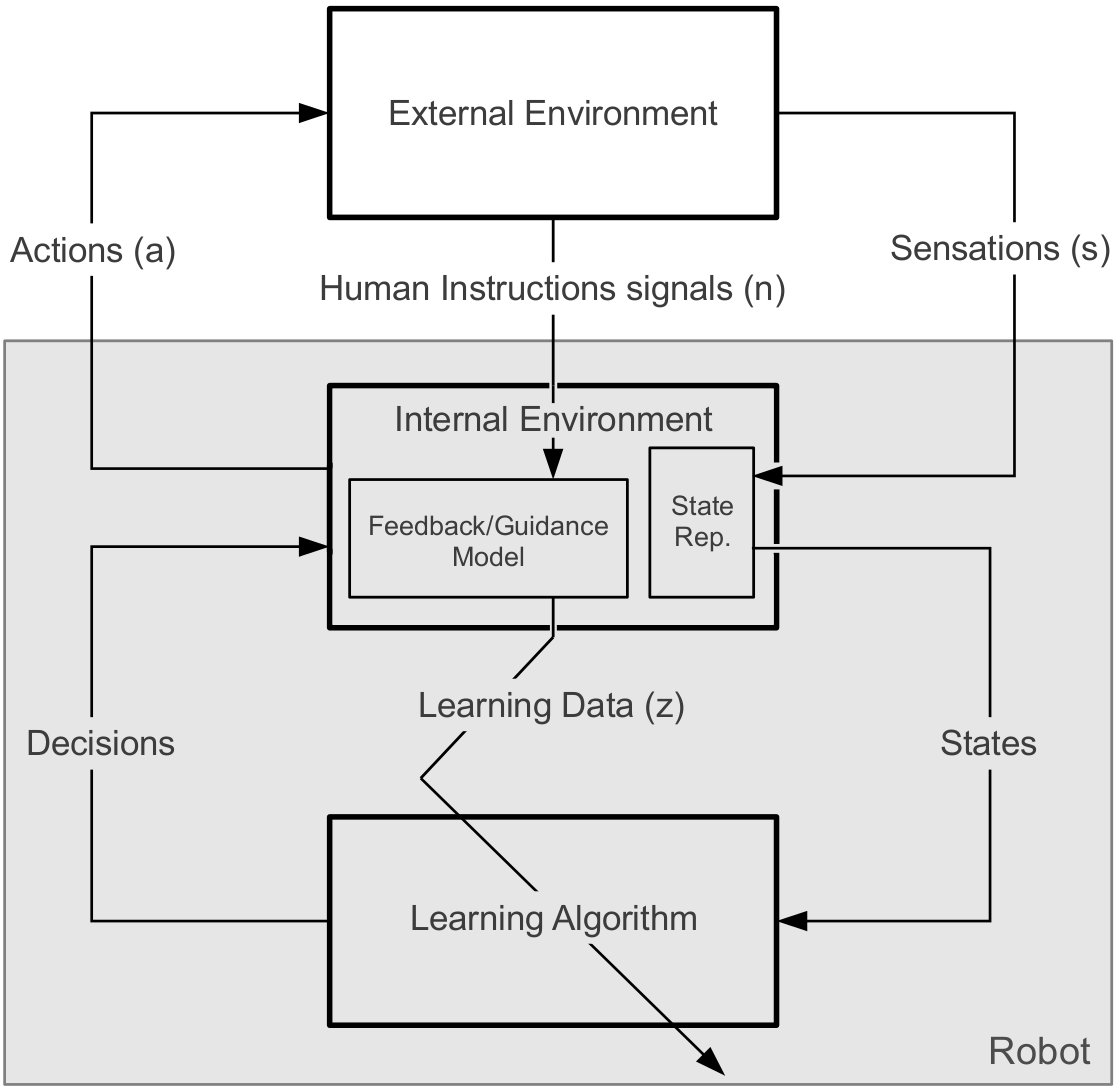
\includegraphics[width=\columnwidth]{images/problem_representation}
           %\caption{Reinforcement learning oriented architecture of our problem. Humans provide teaching signals, which are instructions for learning a task, but which meanings are a priori unknown. The meaning of these signals has to be learnt by the robot in addition to learning the task itself.}
        %\label{fig:ProblemRepresentation} 
   %\end{center}
%\end{figure} 


At home, workplaces or schools, an increasing amount of intelligent robotic systems are starting to be able to help us in our daily life (windows or vacuum cleaners, self-driving cars) \cite{gates2007robot} and in flexible manufacturing systems \cite{baxter}. A key feature in these new domains is the close interaction between people and robots. In particular, such robotic systems need to be teachable by non-technical users, i.e. \textbf{programmable for new tasks in novel environments} through \textbf{intuitive, flexible and personalized interactions}. Specifically, the challenge we address in this work is how a robot learning a new task can be instructed by a human using its own preferred teaching signals, where the mapping between these signals and their meaning is unknown to the robot. For example, different users may use different languages, words, interjections, gestures or even brain signals to mean ``good'' or ``bad''.

While research on robot learning from human interaction has flourished in the last ten years \cite{Argall09lfdsurvey}, most work has focused on how to extract statistical \textit{task models} from human teachers following a fixed pre-defined teaching protocol. Thus, a usual assumption is that the learner and the teacher share a mutual understanding of the meaning of each others' signals. The question of how a robot can learn to interpret personalized and potentially noisy teaching signals, i.e.\ learn \textit{instruction models}, has been much less explored. In a preliminary work \cite{macl11simul}, we presented a computational approach addressing this problem by considering a finite space of teaching signals in simulation while bootstrapping the system with known symbols. Later \cite{grizou2013}, we released the need for bootstrapping and allow the teacher to use any kind of signal that can be represented as a fixed length feature vector, which is better suited for Human-Robot Interaction (HRI) scenario.


Interestingly, a similar approach \cite{Kindermans2012a} has been developed in the Brain Computer Interfaces (BCI) community. Brain-computer interfaces provide a communication channel between humans and machines using only brain activity. Recent works have shown that it is possible to decode information related to human error processing, namely the error-related potentials \cite{FerrezErrores} appearing for instance when the device action does not match the user's expectations. This potential has been used as feedback information to solve sequential tasks \cite{chavarriaga2010learning}\cite{iturrate2010robot}. In practice, BCI solves the meaning problem using an open-loop calibration procedure to train a decoder in a supervised manner. 


In this abstract, we address the problem of removing the need for calibration. We propose an algorithm that simultaneously calibrates the feedback decoder and executes in closed loop a sequential task only known by the user. Our method exploits task constraints, namely optimal policies, to hallucinate the meaning of the teaching signals and select the task with the lowest expected error. We report results from a HRI scenario and a BCI online experiments. The results show that the proposed method is able to learn good feedback models while solving the task efficiently without any calibration.

\section{Methods}

\subsection{BCI control based on feedback signals}

BCI control based on feedback signals differs from classical brain-machine interfaces in the sense that the user does not actively deliver commands to the device, but only delivers feedback about actions performed by the device. In this setting, the device needs to actively execute actions to solve the tasks and to be able to learn an intelligent behavior from the feedback. This idea can be seen as a shared control strategy \cite{millan10}, where both the user and the device help each other to solve a task.

Essentially, this BCI control follows an iterative sequential process where the device performs an action, the user assesses the actions, these assessments are translated into feedback, and the device learns from this feedback. 
%
These assessments are directly related to the error-related potentials, i.e. signals generated when the user observes a device performing a wrong action \cite{FerrezErrores}. After a calibration phase and once a usable decoder is available, user's assessments can be translated into (normally binary) feedback. 
%
This control can be exemplified for a reaching task, where the user wants to reach a target position unknown by the system (see Figure \ref{fig:GM} Top). The device performs several discrete actions (e.g. moving left or right), and learns from the feedback given by the user. After several steps, the device knows which is the desired target and how to reach it.

However, the control can become intractable as the task complexity increases. Furthermore, only binary feedback is available and there is a large percentage of misdetected assessments. Given a set of possible tasks, it is possible to speed up the inference by precomputing the agent's optimal behavior for each task and using the feedback signal as a likelihood for the task.  For instance, in the previous example, the possible tasks is given by the number of targets. An error (negative feedback) after a particular action will decrease the posterior of those targets whose optimal policy agrees with the action. 
%
\subsection{Simultaneous Estimation of Task and Signal Model}
\label{sec:Algorithm}
%
\begin{figure}[!t]%
\centering
\includegraphics[width=0.85	\columnwidth]{images/real_vs_fake}
%\begin{tabular}{cc}
%\includegraphics[width=0.4	\columnwidth]{../figures/1D-ex} &
%\includegraphics[width=0.45	\columnwidth]{../figures/real_vs_fake}\\
%(a) & (b)
%\end{tabular}
\caption{Task labels for a 1-D grid world.  For the represented example, the arrows indicate for each state what action should elicit a positive feedback to reach the target marked with T (i.e., the optimal policies). 2D Gaussian distributions of binary feedback signals for three possible targets are shown below. While for the correct target the distributions shows a large separability (Left), the overlaps increases as the believed target moves away from the real one (Middle, Right). }%}%
\label{fig:GM}%
\end{figure}
%
This section formalizes the problem of executing a task when the feedback meaning is unknown or uncertain.  The main idea is depicted in Fig. \ref{fig:GM} for a toy 1D example. The user wants the device to reach the right-most state. However, neither the target nor the feedback labels are known. The feedback signals are generated as a response to the execution of an action $a$ in state $s$ according to the true unknown task the user wants to solve.  For instance, binary feedback signals as the ones described above simply encode whether the action executed is correct or wrong according to the user.  The key point is that  these signals are generated from an underlying model that for binary signals has two different classes. Given sufficient feedback signals, it is possible to build the underlying distributions for each possible target. Only the right task will provide the right meanings (or labels) to each of the feedback signals (Fig. \ref{fig:GM}~Left), while the other tasks will gradually mix both classes as the task gradually differs more to the original task (Fig. \ref{fig:GM}~Middle-Right), up to the point of almost mirroring the labels when the target is mirrored. In the remainder of this section we show how this property can be exploited to estimate the task and the model generating the feedback signals.

Let denote $e_i\in \mathbf{R}^n$ to the EEG measurements $e$ obtained after the execution of action $a_i$ in state $s_i$. The meaning (or label) $z_i\in\{c,w\}$ of each feedback signal belongs to one of two classes (correct or wrong).   
%
Following the literature \cite{blankertz2010single}, we will model the EEG signals using independent multivariate normal distributions for each class, $\mathcal{N}(\mu_c, \Sigma_c), \mathcal{N}(\mu_w, \Sigma_w)$. We will denote $\theta$ the set of parameters $\{\mu_c, \Sigma_c,\mu_w, \Sigma_w\}$. 

Regarding the tasks, the system has access to a set of task hypotheses $\xi_1,\ldots,\xi_T$ which includes the task the user wants to solve\footnote{If this is not the case, the system will find the most suitable task.}. We do not make any particular assumption on how the task is represented given that for each particular task $\xi$ we are able to compute a policy $\pi$ which represents the probability of choosing a given action $a$ in state $s$, $\pi_{\xi}(s,a) = p(a|s,\xi)$. As mentioned above, these are the policies that, conditioned on the task, provide meanings to the feedback signals of an action-state pair (e.g. in a reaching task, progressing towards the goal will generate correct answers while moving apart from it will generate wrong ones). 

Our goal is to learn which task $\hat{\xi}$ the user wants to solve based on the assessment of the user extracted from EEG measurements collected while executing actions. Thus collected data are in the form $\{(e_i,s_i,a_i),~i~=~1,\ldots,N\}$, i.e. a sequence of states, actions and teaching signals triplets. 
%
Following the discussion of Fig. \ref{fig:GM}, a sensible option to estimate the task $\xi$ is to measure the coherence of the signal model for each possible task using the virtual meanings provided by the target policy. In other words, the best $(\xi,\theta)$ pair would provide the lowest predictive error (perr) on the observed signals $p(e|s,a,\xi,\theta)$. One possible way of solving this problem is to maximize the expected predictive classification rate:
%
\begin{eqnarray}
\hat{\xi},\hat{\theta}&=& argmax_{\xi,\theta} E_e\left( \delta(z(s,a,\xi), z(e,\theta)) \right)
\end{eqnarray}
%
where $\delta()$ is an indicator function, $z(s,a,\xi)$ is the label (wrong or correct) corresponding to the execution of action $a$ in state $s$ under task $\xi$ and $z(e,\theta_{\xi})$ is the label provided by the Gaussian classifier with parameters $\theta_{\xi}$. The expected predictive error can be explicitly written dependent on the task and decoder model:
%
\begin{eqnarray}
E_e\left( \delta(z(s,a,\xi), z(e,\theta)) \right) &=& \sum_{l=c,w} p(z=l|s,a,\xi) p(z=l|e,\theta)
%E_{e \sim \theta,\xi}
\end{eqnarray}
%
where $p(z=l|s,a,\xi)$ representes the probability of the user assigning label $l$ when assesing task $\xi$. We add a noise term to cope with those situations were the user assessment may be wrong. The model is then
%
\begin{equation*}
    p(z=l|s,a,\xi) = \begin{cases}
						   1-\alpha               & if~a = \argmax_a \pi_{\xi}(s,a)\\
						   \alpha             & \text{otherwise}\\
					   \end{cases}
\end{equation*}
%
with $\alpha$ modeling error rate of the user. 
%This variable could be estimated if we new the ground truth. In our case we will use an approximate value, $alpha = 0.1$.
%
The term $p(z=l|e,\theta_{\xi})$ is just the probability of the meaning under the Gaussian model provided by $\theta_{\xi}$
%
\begin{eqnarray}
	p(z=l|e,\theta) &=& 
				\frac{p(e|z=l, \theta)p(z = l)}{\sum_{k=c,w}{p(e|z=k,\theta)p(z=k)}} = \frac{\mathcal{N}(e|\mu_l, \Sigma_l)p(z = l)}{\sum_{k=c,w}{\mathcal{N}(e|\mu_k, \Sigma_k)p(z=k)}}
	\label{eq:dev}
\end{eqnarray}
%
%$p(z=l|e,\theta) = \frac{\mathcal{N}(e|\mu_l, \Sigma_l)}{\sum_{k=c,w} \mathcal{N}(e|\mu_k, \Sigma_k)}$
%I am not sure of the notation $\mathcal{N}(e|\mu_l, \Sigma_l)$ to define the pdf value for $e$
%
%This seems to be how to derive it but not sure
%\begin{eqnarray}
%	p(z=l|e,\theta) &=& \frac{p(z = l,e|\theta)}{p(e|\theta)} \nonumber\\
%				&=& \frac{p(e|z=l, \theta)p(z = l)}{\sum_{k=c,w}{p(e|z=k,\theta)p(z=k)}} \nonumber\\
%				&=& \frac{\mathcal{N}(e|\mu_l, \Sigma_l)p(z = l)}{\sum_{k=c,w}{\mathcal{N}(e|\mu_k, \Sigma_k)p(z=k)}}
%	\label{eq:dev}
%\end{eqnarray}
%With $p(z = c) = p(z = w) = 0.5$
%
Note that the optimization process has be factored using the fact that given the task, the estimation of $\theta$ under the Gaussian model is trivial. It basically requires to compute the maximum-likelihood estimate $\theta^{ML}_{\xi}$ for each target $\xi$. 


